% --- chapter
\newcommand{\chapter}[2][]{
	\newcommand{\chapname}{#2}
	\begin{flushleft}
		\begin{minipage}[t]{\linewidth}
			
\includegraphics[height=1cm]{hdht-logo.png}
			\hspace{0pt}	
			\sffamily\bfseries\large Bài  28. Tia X
			\begin{flushleft}
				\huge\bfseries #1
			\end{flushleft}
		\end{minipage}
	\end{flushleft}
	\vspace{1cm}
	\normalfont\normalsize
}
%-----------------------------------------------------
\chapter[Thang sóng điện từ]{Thang sóng điện từ}

\subsection {Tổng quát về sóng điện từ}
\begin{itemize}
\item Thang sóng điện từ là tập hợp các loại sóng điện từ được sắp xếp theo thứ tự bước sóng tăng (tần số giảm) dần.
\item Các sóng điện từ trong thang sóng điện từ có tần số khác nhau nên tính chất và công dụng của chúng cũng khác nhau.
\end{itemize}
\subsection{Phân loại các sóng điện từ}
\begin{longtable}{|m{4cm}|m{4cm}|m{4cm}|}
	\hline
\thead{Miền sóng điện từ} 	& \thead{Bước sóng (m)} & \thead{Tần số (Hz)} \\
	\hline
Sóng vô tuyến điện & $3 \cdot 10^4 \div 10^{-4}$ & $\thicksim 10^4 \div 3 \cdot 10^{12} $  \\
	\hline
Tia hồng ngoại & $10^{-3} \div \text{7,6} \cdot 10^{-7}$ &  $3 \cdot 10^{11} \div 4 \cdot 10^{14}$\\
	\hline
Ánh sáng nhìn thấy & $\text{7,6}\cdot 10^{-7} \div \text{3,8} \cdot 10^{-7}$  & $4\cdot 10^{14} \div 8 \cdot 10^{14}$  \\
	\hline	
Tia tử ngoại	&$\text{3,8} \cdot 10^{-7} \div 10^{-9}$    & $8\cdot 10^{14} \div 3 \cdot 10^{17}$    \\
	\hline
Tia X & $10^{-8} \div 10^{-11}$& 	$3\cdot 10^{16} \div 3 \cdot 10^{19}$    \\
	\hline
Tia gamma & 	Dưới $10^{-11}$ & Trên $3 \cdot 10^{19}$ \\
	\hline 
\end{longtable}

\begin{center}
	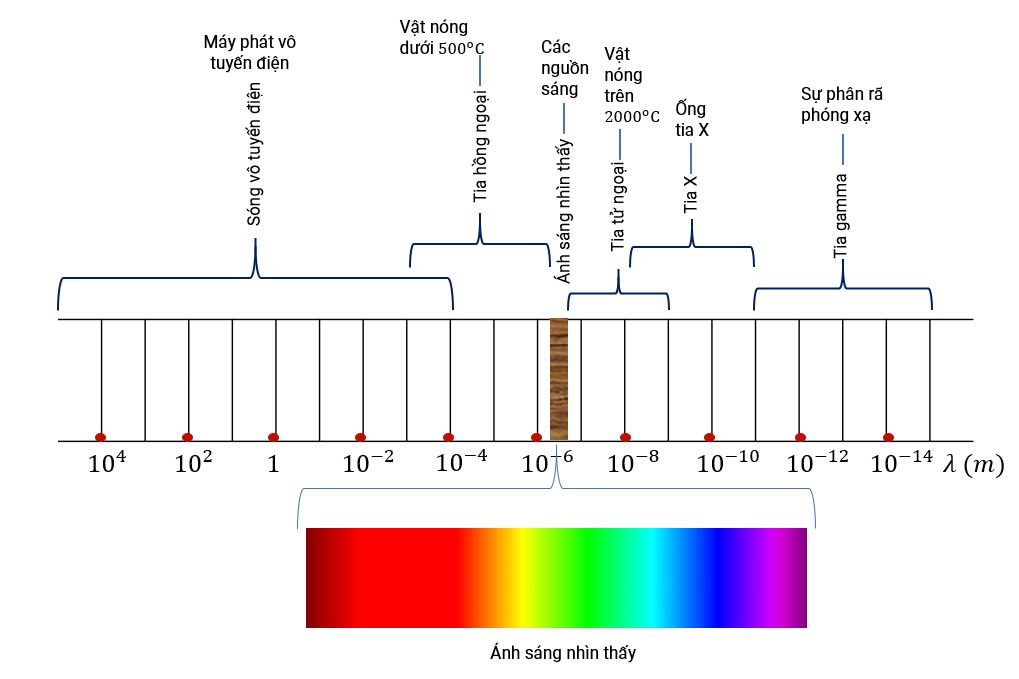
\includegraphics[scale=0.65]{../figs/VN12-PH-36-L-021-6-1.JPG}
\end{center}
